%!TEX root = ../../lod-group1.tex
\subsection{System Architecture}
\label{subsec_method_architecture}

The following section describes the architecture of \emph{Match Forrest, Match!} system.
The central component of the system is the \textit{Task Distributor}.
This component is responsible for managing the other components, \textit{Crawler}, \textit{Triplifier}, \textit{Updater} and \textit{Matcher and Merger}.
It uses a messaging system, which is explained in Section \ref{subsubsec_messaging_infrastructure}.

\subsubsection{System Overview}
\label{subsubsec_workflow}

The overview about the system can be seen in Figure \ref{fig_architecture}.
The first step to get a movie into the system is always to retrieve the web resource about a movie from one of the data sources.
This step is executed by the Crawler.
This component is responsible for downloading websites or for sending requests to the API a data source might provide.

Once the page is downloaded, the Triplifier can triplify the resource.
This means that it extracts the information from the resource (usually in HTML or JSON format) and creates triples according to a certain ontology.
The ontology is described in Section \ref{subsec_method_ontology}.

The component Matcher and Merger is in charge of matching and merging two movies from different data sources, so they can only be found once in the resulting dataset.
This is the crucial step in creating a clean data set.
This component is explained in detail in Section \ref{subsec_method_matching}.

The Updater, described in Section \ref{subsec_method_updating}, ensures that the existing movies are always up-to-date and that new movies are in the system.

The triple store \emph{Virtuoso}\footnote{\url{http://virtuoso.openlinksw.com/}} is used to store the resulting triples.
To distinguish between the sources of the different triples, triples from each data source are stored in a distinct graph named after the source.
Thus, there are four graphs in the triplestore: IMDb, Freebase, TMDb and OFDb.

\begin{figure}[ht]
  \begin{center}
  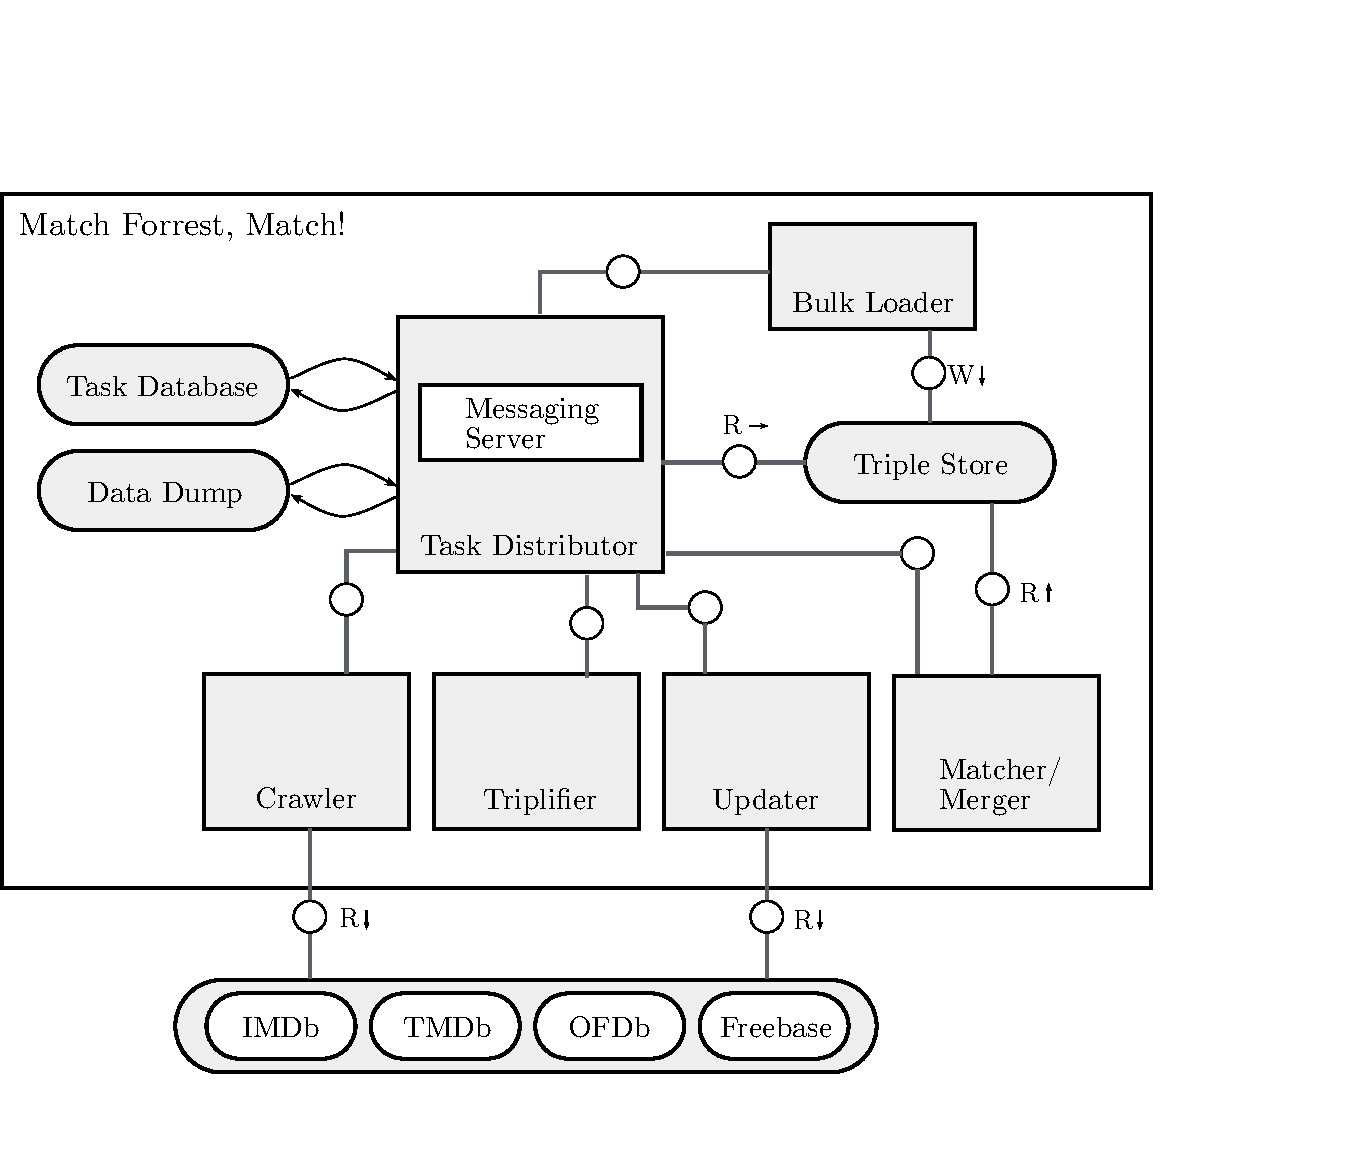
\includegraphics[width=0.8\textwidth]{images/architecture.pdf}
  \end{center}
  \caption{Architecture of \emph{Match Forrest, Match!}. The central component of the system is the Task Distributor, which is responsible for managing the other components, Crawler, Triplifier, Updater and Matcher and Merger.}
  \label{fig_architecture}
\end{figure}

\subsubsection{Messaging Infrastructure}
\label{subsubsec_messaging_infrastructure}

The process of crawling, triplifying and matching a movie resource takes a lot of time.
This is especially true when there are limits to crawl some web pages, which means that waiting times can occur.
Triplifying and matching needs computational resources.
Because these steps can be done in parallel, a messaging infrastructure was implemented to speed up the process and to avoid crawl limits.

Therefore, the Task Distributor uses \emph{RabbitMQ}\footnote{\url{http://www.rabbitmq.com/}} to coordinate and send created task to multiple workers.

A task consists of the following fields
\begin{itemize}
  \item \textbf{Id}:
  The unique id of the task.
  \item \textbf{Task type}:
   The type of the task.
  Basically there is a type for each of the compontents, controlled by the Task Distributor, for example ``Triplify'' or ``MatchAndMerge''.
  ``Triplify'' is a task executed by the Triplifier component.
  The Matcher and Merger component works on ``MatchAndMerge'' tasks.
  There are also tasks, which combine some steps, e.g. one task which crawls, triplifies and matches a movie. This is important for updating, since then all of them are better done at once.
  \item \textbf{Due date}:
  The date until when the task should be finished.
  \item \textbf{File or URL}:
  The file or url which is needed to execute the task, e.g. a URL to crawl or a JSON file to triplify.
  \item \textbf{Finished:}
  Defines if the task is already done.
  \item \textbf{Graph}:
  The graph in which the resulting triples should be stored.
  \item \textbf{Special flags}:
  Additional information needed when executing a task.
  For example, it could tell whether a certain entity should be deleted from the triple store before storing new triples.
\end{itemize}
Not all fields have to be set, the task type defines which fields are needed.
For example the ``Triplify'' task needs a file, but the ``MatchAndMerge'' task does not.

All tasks are stored in an SQL database and new ones are created by the Updater.
To get an initial data set, tasks have to be created manually.

The messaging server takes a task from the SQL database and puts it into the messaging queue.
The functionality of the messaging system, is shown in Figure \ref{fig_messaging_infrastructure}.
The new task is then pushed to a worker which is registered on the task queue.
If multiple workers are registered, a free worker is selected by using the round robin principle to perform the next task.
When the worker has finished the task, it sends its answer to the answer queue and waits for the server to acknowledge its work.
The server receives the worker's answer from the answer queue and then stores given triples into the triple store or files into the file system.
When the answer was successfully stored, the server sends his acknowledgement to the worker who forwards the acknowledgement to the task queue.
The task is now successfully executed and the worker can work on the next task in the task queue.
If an acknowledgement takes longer than a certain time, the task would be assigned to another worker.
This ensures that no tasks get lost.
By only sending the acknowledgement after storing the data, it is also ensured that only really finished tasks are considered as finished.

\begin{figure}[ht]
  \begin{center}
  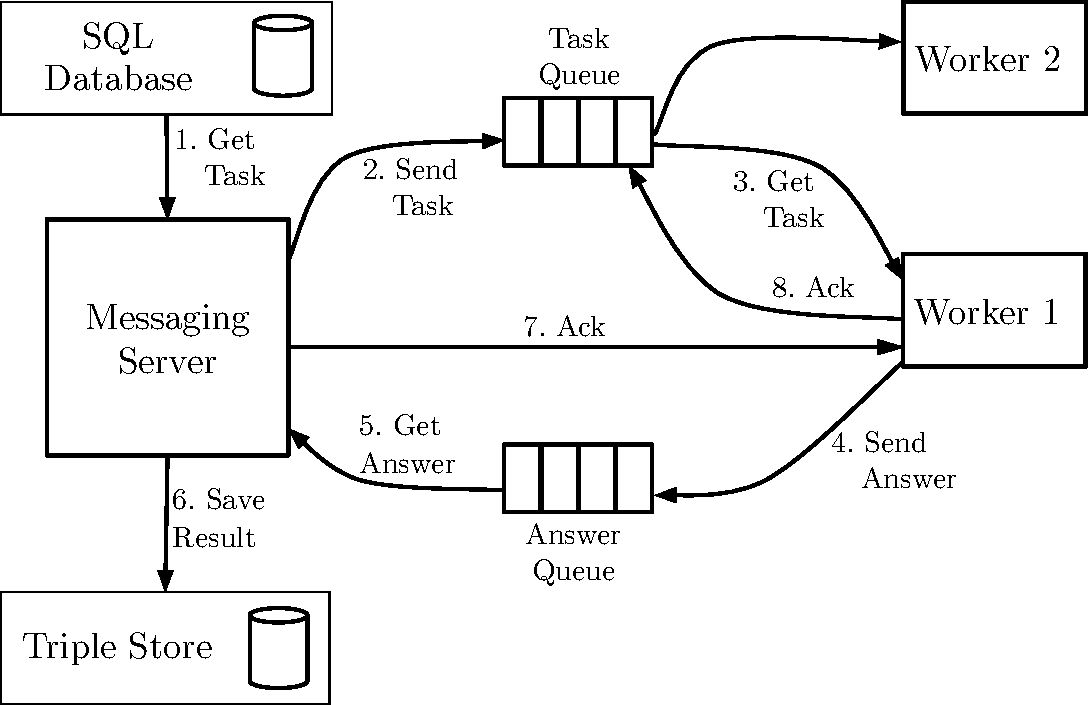
\includegraphics[width=0.7\textwidth]{images/rabbit_mq.pdf}
  \end{center}
  \caption{Messaging Infrastructure using RabbitMQ.}
  \label{fig_messaging_infrastructure}
\end{figure}